\section{Auswertung}

\subsection{Überprüfung der Bragg-Bedingung}

Bei einem Kristallwinkel von $\theta_{\text{K}} = 14{\textdegree}$ wurde der Winkel $\theta_{\text{GM}}$ vom Geiger-Müllerzählrohr variiert und die Zählrate gemessen.
Die Werte sind in der Tabelle \ref{tab:ogemessdaten1} angegeben und lassen sich nun in ein Diagramm \ref{fig:plot1} mit Winkelabhängigkeit einzeichnen.
\begin{figure}[h]
  \centering
  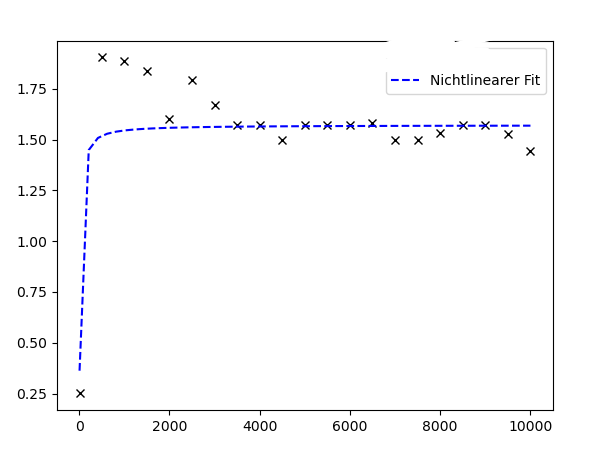
\includegraphics[width=\textwidth]{build/plot1.pdf}
  \caption{Zählratendiagramm mit Winkelabhängigkeit.}
  \label{fig:plot1}
\end{figure}
Der Winkel mit der höchsten Zählrate lässt sich am Diagramm \ref{fig:plot1} und an den Messwerten \ref{tab:ogemessdaten1} als
\begin{equation}
\theta_{\text{max}} = 28{,}2{\textdegree}
\end{equation}
feststellen.
Die theoretische Lage des Maximums ist bei fest eingestellten 14$\textdegree$ des Kristalls genau das doppelte. Also hat der Sollwert einen Winkel von $\theta_{\text{soll}} = 28{\textdegree}$. Es ergibt sich folgende Abweichung vom Sollwert.
\begin{equation}
\increment \theta = \theta_{\text{max}} - \theta_{\text{soll}} = 0{,}2{\textdegree}
\end{equation}

\subsection{Analyse eines Emissionsspektrums einer Kupfer-Röntgenröhre}

Das Emissionsspektrum wurde mit einer Integrationszeit von $\increment t = \SI{10}{\second}$ in jeweils $\increment \theta = 0{,}1\textdegree$ Abständen gemessen.
Die ermittelten Zählraten sind poissonverteilt, somit lässt sich der Fehler gemäß
\begin{equation}
\increment N_{i} = \sqrt{N_{i}}
\end{equation}
berechnen. Diese Werte lassen sich nun mit einem Fehlerbalken in ein Diagramm \ref{fig:plot2} eintragen wobei die Charakteristik des Zählrohrs gut zu erkennen ist.
Der Bremsberg ist im Diagramm durch schwarze Punkte dargestellt, sie zeigen die Strahlung welche durch Abbremsung der Elektronen am Kupfer entsteht. 
Außerdem sind zwei charakteristische Linien zu erkennen, die $K_{\beta}$ und $K_{\alpha}$-Linie. 
Die Maxima dieser Linien liegen bei.
\begin{align}
K_{\alpha} &= 20{,}2\textdegree \\
K_{\beta} &= 22{,}5\textdegree
\end{align}
Sie zeigen jeweils die Winkeleinstellung, bei der ein Photon durch das zurückfallen eines Elektrons auf eine
niedrigere Schale, in dem Fall von $n=2$ auf $n=1$ für $K_{\alpha}$ und von $n=3$ auf $n=1$ für $K_{\beta}$, am Kristall reflektiert wird. 
An den ermittelten Werten lässt sich keine minimale Wellenlänge und keine maximale Energie des Bremsbergs bestimmen. Für Information auf die minimale Wellenlänge müsste bei einer geringe Winkeleinstellung
gemessen werden damit der Punkt sichtbar wird, wo die Zählrate noch auf Null steht. Der Bremsberg verläuft relativ linear in dem gemessenen Winkelbereich und fällt nur schwach ab, daraus lässt sich kein
aussagekräftiges Maximum erkennen. 
\subsubsection{Halbwertsbreite}
Für jede charakteristische Linie kann eine Halbwertsbreite ermittelt werden, dazu wird das Intensitätsmaximum halbiert und die Werte links und rechts neben dem Maximum die diesen Wert
annehmen bestimmen die Halbwertsbreite.
Zunächst hat $K_{\beta}$ eine halbierte Peakintensität von $N_{\beta} = \SI{2525}{{\text{Imp}}\per\second}$ die gemessenen Werte liegen zwischen diesem Wert, deshalb kann eine
lineare Approximation verwendet werden. Es gilt.
\begin{equation}
2525 = \frac{P_{2}-P_{1}}{0{,}1} \cdot \theta + P_{1}
\end{equation}
Dabei ist $P_{2}$ der Punkt der gerade über der halben Peakintensität ist und $P_{1}$ der, welcher gerade darunter liegt.
Dies kann nach $\theta$ umgeformt werden und auf den Wert $\theta_{P_{1}}$ addiert werden. Es ergibt sich also der Punkt der Halbwertsbreite links vom Maximum.
\begin{equation}
\theta_{\text{links}} = 0{,}1 \cdot \frac{2525-P_{1}}{P_{2}-P_{1}} + \theta_{P_{1}}
\end{equation}
Es ergeben sich die Werte.
\begin{align}
\theta_{K_{\beta}\text{,links}} &= 22{,}35\textdegree\\
\theta_{K_{\beta}\text{,rechts}} &= 22{,}85\textdegree
\end{align}
Für die rechte Seite muss dabei beachtet werden, dass sich das Vorzeichen der Steigung ändert.
Die Halbwertsbreite für $K_{\beta}$ ist also.
\begin{equation}
\text{FWHM}_{K_{\beta}} = \theta_{K_{\beta}\text{,rechts}} - \theta_{K_{\beta}\text{,links}} = 0{,}5\textdegree
\end{equation}
FWHM steht dabei für \enquote{Full Width at Half Maximum}.
Mit einer analogen Rechnung für $K_{\alpha}$ ergeben sich die folgenden Werte.
\begin{align}
\theta_{K_{\alpha}\text{,links}} &= 20{,}06\textdegree \\
\theta_{K_{\alpha}\text{,rechts}} &= 20{,}55\textdegree \\
\text{FWHM}_{K_{\alpha}} &= 0{,}49\textdegree
\end{align}
Die Halbwertsbreiten sind ebenfalls in das Diagramm \ref{fig:plot2} eingezeichnet.
\begin{figure}[h]
  \centering
  \includegraphics[width=\textwidth]{build/plot2.pdf}
  \caption{Röntgenspektrum einer Kupfer-Röntgenröhre.}
  \label{fig:plot2}
\end{figure}
\subsubsection{Auflösevermögen}
Für das Auflösevermögen müssen die Energien der charakteristischen Linien $E_{K}$ bestimmt werden, sowie die Energiedifferenz der Halbwertsbreiten $\increment E_{\text{FWHM}}$.
Das Auflösevermögen $A$ lässt sich durch
\begin{equation}
\label{eqn:gg}
A = \frac{E_{K}}{\increment E_{\text{FWHM}}}
\end{equation}
errechnen. Die Energien lassen sich nach der Gleichung \eqref{eqn:braggEnergy} bestimmen.
Die folgende Wertetabelle gibt die Ergebnisse an.
\begin{table}
\centering
\caption{Energien der charakteristischen Linien zur Bestimmung des Auflösevermögen.}
\label{tab:lol}
\begin{tabular}{c c c c c}
    \toprule
    Linie & $E_{\text{peak}}$[$\si{\kilo\electronvolt}$] & $E_{\text{FWHM,links}}$[$\si{\kilo\electronvolt}$] & $E_{\text{FWHM,rechts}}$[$\si{\kilo\electronvolt}$] & $\increment E_{\text{FWHM}}$[$\si{\kilo\electronvolt}$] \\
    \midrule
    $K_{\alpha}$ & $\SI{8.043}{}$& $\SI{8.974}{}$& $\SI{8.769}{}$ & $\SI{205.045}{}$\\
    $K_{\beta}$ &$\SI{8.914}{}$ &$\SI{8.095}{}$ &$\SI{7.927}{}$ & $\SI{167.938}{}$ \\
    \bottomrule
\end{tabular}
\end{table}
Diese Werte lassen sich nun in die Gleichung \eqref{eqn:gg} einsetzen und es folgen zwei Werte des Auflösevermögens für die beiden Linien.
\begin{align}
A_{K_{\alpha}} &= 39.227 \\
A_{K_{\beta}} &= 53.080
\end{align}

\subsubsection{Bestimmung der Abschirmkonstanten}
Aus den Gleichungen \eqref{eqn:sommerfeldenergie} und \eqref{eqn:kackeq} lassen sich bei Vernachlässigung des Drehimpulsbeitrages die Abschirmkonstanen für Kupfer folgendermaßen angeben.
\begin{align}
\label{eqn:11}
\sigma_1 &= Z_{\text{Cu}} - \sqrt{\frac{E_{\symup{K,abs}}}{R_{\infty}} } \\
\sigma_2 &= Z_{\text{Cu}} - 2 \sqrt{\frac{R_{\infty}(z - \sigma_1)^2 - E_{\symup{\alpha}}}{R_{\infty}}} \\
\label{eqn:33}
\sigma_3 &= Z_{\text{Cu}} - 2 \sqrt{\frac{R_{\infty}(z - \sigma_1)^2 - E_{\symup{\beta}}}{R_{\infty}}} 
\end{align}
Für die Berechnung von $\sigma_1$ wird die Absorptionsenergie der K-Kante benötigt hierzu wird ein Literaturwert zur Rate gezogen.
Dieser ist nach \cite{random}.
\begin{equation}
E_{\symup{K,abs}} = \SI{8987.96(15)}{\electronvolt}
\end{equation}
Dieser Wert kann nun zusammen mit den bereits bestimmten Energien an den Peaks der $K_{\alpha}$ und $K_{\beta}$-Linie aus Tabelle \ref{tab:lol} in die Gleichungen \eqref{eqn:11} bis
\eqref{eqn:33} eingesetzt werden.
\begin{align}
\sigma_1 &= \SI{3.2978(2)}{}\\
\sigma_2 &= \SI{12.3354(13)}{}\\
\sigma_3 &= \SI{24.3434(47)}{}
\end{align}
